\documentclass[12pt]{article}
%Also I made it 12pt

\usepackage[fontset=macnew]{ctex}
\usepackage{physics}
\usepackage{tikz}
\usetikzlibrary{3d,calc,patterns}
% \usepackage{tkz-euclide}
\usepackage{amsmath}
\usepackage{upgreek}
\usepackage{amsthm}
\usepackage{amsfonts}
%to add an affiliation line to the the title formatting
\usepackage{authblk}

%Fonts
% \usepackage[no-math]{fontspec} %This allows you to enter (via an IPA kayboard) IPA fonts and other symbols directly into LaTeX. Requires a particular setyp, see below.
\usepackage{libertine} %A font that actually contains many IPA symbols. This is the font you see in the preview to the right.

%to use these fonts, be sure that your typesetting engine is set to "XeLaTeX." In Overleaf, go to the Menu link on the top left (by the Overleaf icon), and under Settings be sure that the Compiler is set to "XeLaTeX." If you accessed this document via the Overleaf Pomona Linguistics template, all of this was already done for you.

%The Pomona Linguistics Paper Template in Overleaf is already set up for this, but you may run into this problem if you start building your own documents.


%%%%%%%%%%%%%%%%%%%%%%%%%%%%%%%%%%%%%%%%%%%%%%%%%%%
%packages for this style of handout-formatting of (sub)section headers 
\usepackage[explicit]{titlesec}
\usepackage{xcolor}

\definecolor{light-gray}{gray}{0.7}
\definecolor{lighter-gray}{gray}{0.85}

\titleformat{\section}
{\normalfont\Large\bfseries}{}{0em}{\colorbox{black}{\parbox{\dimexpr\textwidth-2\fboxsep\relax}{\textcolor{white}{\thesection\quad#1}}}}

\titleformat{\subsection}
{\normalfont\large\bfseries\scshape}{}{0em}{\colorbox{light-gray}{\parbox{\dimexpr\textwidth-2\fboxsep\relax}{\textcolor{black}{\thesubsection\quad#1}}}}

\titleformat{\subsubsection}
{\normalfont\bfseries}{}{0em}{\colorbox{lighter-gray}{\parbox{\dimexpr\textwidth-2\fboxsep\relax}{\textcolor{black}{\thesubsubsection\quad#1}}}}
%%%%%%%%%%%%%%%%%%%%%%%%%%%%%%%%%%%%%%%%%%%%%%%%%%%

%%% This file is the preamble for the Pomona Linguistics LaTeX Paper Template, which is also used for the Quick Reference Guide. If you are brand new to writing with LaTeX, we suggest NOT messing with it, and just writing your paper using the Paper Template. If you are getting more comfortable in LaTeX and want to add packages and commands, this is where you do it (when using this template).

%For stacking text, used here in autosegmental diagrams
\usepackage{stackengine}

%To combine rows in tables
\usepackage{multirow}

%geometry helps manage margins, among other things.
\usepackage[margin=1in]{geometry}

%Gives some extra formatting options, e.g. underlining/strikeout
\usepackage{ulem}

%For putting links into papers, also helps make cross-references in the paper smart references
\usepackage[colorlinks = true,
            linkcolor = blue,
            urlcolor  = blue,
            citecolor = blue,
            anchorcolor = blue]{hyperref} %smarter cross-references, these options turn links blue

%Use package/command below to create a double-spaced document, if you want one. Uncomment BOTH the package and the command (\doublespacing) to create a doublespaced document, or leave them as is to have a single-spaced document.
%\usepackage{setspace}
%\doublespacing 

%paragraph formatting
\usepackage[parfill]{parskip}
\setlength{\parskip}{5pt} %plus 1 minus 1}
\setlength{\parindent}{30pt}
\usepackage{titlesec}

%use for special OT tableaux symbols like bomb and sad face. must be loaded early on because it doesn't play well with some other packages
\usepackage{fourier-orns}

%Basic math symbols 
\usepackage{pifont}
\usepackage{amssymb}

%%%Gives shortcuts for glossing. The use of this package is NOT explained in the Quick Reference Guide, but the documentation is on CTAN for those that are interested. MJKD finds it handy for glossing. (https://ctan.org/pkg/leipzig?lang=en)
\usepackage{leipzig}

%Tables
\usepackage{caption} %For table captions
\usepackage{booktabs} %helps format tables

%For citations and bibliography - as of 9.1.2019 we don't explain citations in this Quick Reference Guide, but Pedro Martin's tutorial does (see links in the Guide).
\usepackage{natbib}

%For OT-style tableaux
\usepackage{ot-tableau}

%highlights text with \hl{text}
\usepackage{color, soul}

%Drawing Syntax Trees
\usepackage[linguistics]{forest}

%This specifies some formatting for the forest trees to make them nicer to look at
\forestset{
  nice nodes/.style={
    for tree={
      inner sep=0pt,
      fit=band,
    },
  },
  default preamble=nice nodes,
}

%% For numbered and glossed examples %%
\usepackage{gb4e}



%Changes the \maketitle command to be smaller and take up less space on a page. 
\makeatletter         
\def\@maketitle{   % custom maketitle 
\noindent {\Large \bfseries \color{black} \@title}  \\ \hrule \noindent \@author \\ \@date  
}

%The code below will draw a circle around a piece of text. This is very useful for drawing attention to a word in a data example. use the command \circled{text} where the argument (`text' here) is what you want to be circled. This is illustrated in the Quick Reference Guide and the Paper Template.

\usepackage{tikz}

\newcommand{\circled}[1]{\begin{tikzpicture}[baseline=(word.base)]
\node[draw, rounded corners, text height=8pt, text depth=2pt, inner sep=2pt, outer sep=0pt, use as bounding box] (word) {#1};
\end{tikzpicture}
}


%%%%%%%%%%%%%%%%%%%%%%%%%%%%%%%%%%%%%%%%%%%%%%%%%%%%%%%%%%%%
%%%%%%%%%%%%%%%%%%%%%%%%%%%%%%%%%%%%%%%%%%%%%%%%%%%%%%%%%%%%

% Useful Ling Shortcuts

\RequirePackage{leipzig}
%\RequirePackage{mathtools} % for \mathrlap

% % % Shortcuts  (borrowed from JZ, I'm still unsure exactly what xspace requires)
\RequirePackage{xspace}
\xspaceaddexceptions{]\}}

%This makes the \emptyset command be a nicer one
\let\oldemptyset\emptyset
\let\emptyset\varnothing
\newcommand{\nothing}{$\emptyset$}

%Not all of these are explained in the Quick Reference Guide, but they are here bc they are relevant to some of our students.
\newcommand{\1}{\rlap{$'$}\xspace}
\newcommand{\0}{\rlap{\textsuperscript{$ˆ{\circ}$}}\xspace}
\newcommand{\Lb}[1]{$\text{[}_{\text{#1}}$ } %A more convenient left bracket
\newcommand{\Rb}[1]{$\text{]}_{\text{#1}}$ } %A more convenient left bracket
\newcommand{\gap}{\underline{\hspace{1.2em}}}
\newcommand{\vP}{\emph{v}P}
\newcommand{\lilv}{\emph{v}}
\newcommand{\Abar}{A$'$-} %A more convenient A-bar notation
\newcommand{\ph}{$\varphi$\xspace} %A more convenient phi
\newcommand{\pro}{\emph{pro}\xspace}
\newcommand{\subs}[1]{\textsubscript{#1}} %A more convenient subscript
%\newcommand{\hd}{$^{\circ}$\xspace} %Symbol for printing head / degree symbol
\newcommand{\spells}{$\Longleftrightarrow$} %spellout arrow for morph spellout rules
% \newcommand{\tr}[1]{\textit{t}\textsubscript{\textit{#1}}} %easy traces with subscript
\newcommand{\supers}[1]{\textsuperscript{#1}}

% Abbreviations for glossing, based on Leipzig
\newleipzig{hab}{hab}{habitual}
\newleipzig{rem}{rem}{remote}
\newleipzig{sm}{sm}{subject marker}
\newleipzig{t}{t}{tense}
\newleipzig{aa}{aa}{anti-agreement}
\newleipzig{pron}{pron}{pronoun}
\newleipzig{rec}{rec}{recent}
\newleipzig{om}{om}{object marker}
%\newleipzig{ipfv}{ipfv}{imperfective}
\newleipzig{asp}{asp}{aspect}
\newleipzig{lk}{lk}{linker}
\newleipzig{pcl}{pcl}{particle}
\newleipzig{stat}{stat}{stative}
\newleipzig{ints}{ints}{intensive}
\newleipzig{ascl}{ascl}{assertive subject clitic}
\newleipzig{nascl}{nascl}{non-assertive subject clitic}
\newleipzig{ta}{ta}{tense and/or aspect}
\newleipzig{assoc}{assoc}{associative marker}
\newleipzig{hon}{hon}{honorific}
%\newleipzig{whprt}{wh}{\wh particle}
\newleipzig{sa}{sa}{subject agreement}
\newleipzig{conj}{conj}{conjunction}
%\newleipzig{loc}{loc}{locative}
\newleipzig{expl}{expl}{expletive}
\newleipzig{rcm}{rcm}{reciprocal marker}
\newleipzig{pers}{pers}{persistive}
%\newleipzig{}{}{} %this is just to copy for when I want to add more

%%%%%%%%%%%%%%%%%%%%%%%%%%%%%%%%%%%%%%%%%%%%%%%%%%%%%%%%%%%%
%%%%%%%%%%%%%%%%%%%%%%%%%%%%%%%%%%%%%%%%%%%%%%%%%%%%%%%%%%%%

%A couple of packages that seemed to prefer being called toward the end of the preamble

%This package provides macros for typesetting SPE-style phonological rules.
\usepackage{phonrule}

%For using Greek letters outside of math mode.
\usepackage{textgreek}


%Random, lets us use the XeLaTeX logo. Not important to the template at all.
\usepackage{metalogo}


%%%%%%%%%%%%
%% This is the end of the PREAMBLE
%%%%%%%%%%%

%MJKD note to future self - this preamble is just the section headers + PomLing formatting, but an ordering paradox between the two files made me combine them and re-order fontspec. *shrug* In future if it needs an update, just take the PomLing formatting file and add in the section headers for handouts.

\newcommand{\rmd}{\mathrm{d}}
\newcommand{\deriv}[2]{\frac{\rmd #1}{\rmd #2}}
\newcommand{\pderiv}[2]{\frac{\partial #1}{\partial #2}}
\newcommand{\dpderiv}[2]{\dfrac{\partial #1}{\partial #2}}
\newcommand{\dderiv}[2]{\dfrac{\rmd #1}{\rmd #2}}

\title{磁介质}
\author{\href{mailto:lai-wei@whu.edu.cn}{Lai Wei}}
\date{\today}

\begin{document}

\maketitle
 
\section{磁介质的磁化}

\subsection{磁介质的磁化 \quad 相对磁导率}

被磁化后的磁介质会激发附加磁场\(\boldsymbol{B^\prime}\),从而影响介质内外的磁场分布。磁介质内的磁感应强度为
\begin{equation}
    \boldsymbol{B} = \boldsymbol{B_0} + \boldsymbol{B^ \prime}
\end{equation}

相对磁导率
\begin{equation}
    \mu_r = \frac{B}{B_0}
\end{equation}

相对磁导率\(\mu_r\)的大小只与磁介质的性质有关,根据\(\mu_r\)的大小将磁介质分成顺磁质、抗磁质和铁磁质三类。

\begin{enumerate}
    \item 顺磁质\(\mu_r\)略大于1,即\(\mu_r \approx 1 + 10^{-4} > 1\)
    \item 抗磁质\(\mu_r\)略大于1,即\(\mu_r \approx 1 - 10^{-5} < 1\)
    \item 铁磁质\(\mu_r >> 1\),磁化后产生的磁场\(\boldsymbol{B^\prime}\)的方向与原磁场\(\boldsymbol{B_0}\)的方向相同,且\(\boldsymbol{B^\prime} >> \boldsymbol{B_0}\)
\end{enumerate}

\subsection{磁化强度和磁化电流}

将磁介质中单位体积内分子磁矩的矢量和称为\emph{磁化强度},并用\(\boldsymbol{M}\)来表示,即
\begin{equation}
    \boldsymbol{M} = \frac{\sum \boldsymbol{m_{\text{分子}}}}{\Delta V} = \frac{\sum \boldsymbol{m} + \sum \Delta \boldsymbol{m}}{\Delta V}
\end{equation}
在国际单位制中,\(\boldsymbol{M}\)的单位为\(\mathrm{A} \cdot \mathrm{m}^{-1}\)。

设有一“无限长”的载流直螺线管,管内充满均匀磁介质,电流在螺线管内激发匀强磁场。在此磁场中磁介质被均匀磁化,这时磁介质中各个分子电流平面将转到与磁场的方向相垂直。对磁介质的整体来说,未被抵消的分子电流是沿着柱面流动的,称为安培表面电流(或叫磁化面电流),用\(I_s\)表示。沿轴线单位长度上的磁化电流称为磁化电流密度,用\(\boldsymbol{j_s}\)表示。于是,沿棒的轴线方向长为\(L\)的表面上,磁化电流的大小为\(I_s = j_s L\)。介质被磁化的程度越大,介质表面的磁化电流越大。

\begin{figure}[!h]
    \centering
    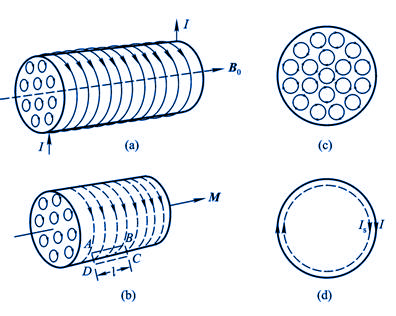
\includegraphics[width = .4\textwidth]{graphics/磁化电流.png}
\end{figure}

对顺磁性物质,安培表面电流和螺线管上导线中的电流方向相同;对抗磁性物质,则两者方向相反。

即当磁化强度的方向与介质表面平行时,磁介质表面磁化电流密度的大小等于该处磁化强度的大小,即
\begin{equation}
    M = \frac{\sum  \boldsymbol{m}_{\text{分子}}}{\Delta V} = \frac{j_s L S}{L S} = j_s
\end{equation}

如果磁化强度的方向与介质表面不平行,可以证明
\begin{equation}
    \boldsymbol{j}_s = \boldsymbol{M} \times \boldsymbol{e}_n
\end{equation}
式中\(\boldsymbol{e}_n\)为磁介质表面的外法线单位矢量。该式表明,磁化强度\(\boldsymbol{M}\)沿磁介质表面的切向分量等于介质表面的磁化电流密度。

可以证明:磁化强度\(\boldsymbol{M}\)与磁化电流\(I_s\)之间的普遍关系为
\begin{equation}
    \oint_L \boldsymbol{M} \cdot \rmd \boldsymbol{L} = \sum I_s
    \label{13-6}
\end{equation}

\section{有磁介质存在时的安培环路定理和高斯定理}

\subsection{有磁介质存在时的安培环路定理 \quad 磁场强度}

有磁介质存在时,空间任意一点的磁感应强度\(\boldsymbol{B}\)应由导线中的传导电流\(I_0\)和磁介质表面的磁环电流\(I_s\)共同产生,因此有磁介质存在时,磁场的安培环路定理应写成
\begin{equation}
    \oint_L \boldsymbol{B} \cdot \rmd \boldsymbol{L} = \mu_0 \left(\sum I_0 + \sum I_s\right)
\end{equation}
式中,\(\sum I_0\)是穿过闭合回路\(L\)所围面积的传导电流的代数和,\(\sum I_s\)时磁化电流的代数和。

如果将磁化强度\(\boldsymbol{M}\)与磁化电流\(I_s\)的普遍关系式\ref{13-6}代入上式,则有
\begin{equation}
    \oint_L \boldsymbol{B} \cdot \rmd \boldsymbol{L} = \mu_0 \left(\sum I_0 + \oint_L \boldsymbol{M} \cdot \rmd \boldsymbol{L}\right)
\end{equation}
或写为
\begin{equation}
    \oint_L \left(\frac{\boldsymbol{B}}{\mu_0} - \boldsymbol{M}\right) \cdot \rmd \boldsymbol{L} = \sum I_0
    \label{13-9}
\end{equation}

引入一个新的辅助物理量,称为\emph{磁场强度},用\(\boldsymbol{H}\)表示,并定义
\begin{equation}
    \boldsymbol{H} = \frac{\boldsymbol{B}}{\mu_0} - \boldsymbol{M}
\end{equation}
则式\ref{13-9}可写为
\begin{equation}
    \oint_L \boldsymbol{H} \cdot \rmd \boldsymbol{L} = \sum I_0
    \label{13-11}
\end{equation}

式\ref{13-11}称为有磁介质时的安培环路定理,它表明磁场强度\(\boldsymbol{H}\)沿任一闭合回路\(L\)的线积分(或环流)等于通过该回路\(L\)所围成面积的传导电流的代数和。

\subsection{磁介质的磁化特性}

在各向同性的磁介质内部,任意一点的磁化强度\(\boldsymbol{M}\)和磁场强度\(\boldsymbol{H}\)成正比,即
\begin{equation}
    \boldsymbol{M} = \chi_m \boldsymbol{H}
\end{equation}
式中\(\chi_m\)为比例系数,称为介质的\emph{磁化率},对于顺磁质,\(\chi_m > 0\),表明顺磁质中\(\boldsymbol{M}\)和\(\boldsymbol{H}\)的方向相同;对于抗磁质,\(\chi_m > 0\),表明抗磁质中\(\boldsymbol{M}\)和\(\boldsymbol{H}\)的方向相反。

于是
\begin{equation}
    \boldsymbol{B} = \mu_0 (1 + \chi_m)\boldsymbol{H} = \mu_0 \mu_r \boldsymbol{H}= \mu \boldsymbol{H}
\end{equation}
式中
\begin{equation}
    \mu_r = 1 + \chi_m, \quad \mu = \mu_0\mu_r
\end{equation}
\(\mu_r\)和\(\mu_0\)分别称为磁介质的相对磁导率和绝对磁导率(有时也简称为磁导率)。

对于真空中的磁场,由于\(\boldsymbol{M} = 0\),则\(\chi_m = 0\),\(\boldsymbol{B} = \mu_0 \boldsymbol{H}\),这表明真空的相对磁导率\(\mu_r = 1\)。

\subsection{有磁介质存在时的高斯定理}

\begin{equation}
    \oint_S \boldsymbol{B} \cdot \rmd \boldsymbol{S} = 0
\end{equation}

\end{document}